% !TEX encoding = UTF-8 Unicode
%\documentclass[handout]{beamer}
\documentclass[bigger,handout]{beamer}
\usetheme{Boadilla}
% !TEX encoding = UTF-8 Unicode
% ÄÖÜ ß äöü



\usepackage[utf8]{inputenc}			% Eingabekodierung
\usepackage[ngerman,english]{babel}	% Unterstütze deutsch und englisch, english ist aktiv, \selectlanguage{ngerman}
\usepackage[T1]{fontenc}				% Korrekte Umlaute im PDF

%\usepackage{ucs}
\usepackage{blindtext}				% Blindtext einfach erzeugen
\usepackage{listings}
\usepackage{floatflt}
\usepackage{color}

%\lstset{
%extendedchars=\true,
%inputencoding=utf8x
%}

\lstset{
extendedchars=\true,
language=XML,                             % Code langugage
basicstyle=\ttfamily,                   % Code font, Examples: \footnotesize, \ttfamily
%keywordstyle=\color{OliveGreen},        % Keywords font ('*' = uppercase)
keywordstyle=\color{blue},        % Keywords font ('*' = uppercase)
commentstyle=\color{red},              % Comments font
numbers=left,                           % Line nums position
numberstyle=\tiny,                      % Line-numbers fonts
stepnumber=1,                           % Step between two line-numbers
numbersep=5pt,                          % How far are line-numbers from code
%backgroundcolor=\color{lightlightgray}, % Choose background color
frame=none,                             % A frame around the code
tabsize=2,                              % Default tab size
captionpos=b,                           % Caption-position = bottom
breaklines=true,                        % Automatic line breaking?
breakatwhitespace=false,                % Automatic breaks only at whitespace?
showspaces=false,                       % Dont make spaces visible
showtabs=false,                         % Dont make tabls visible
columns=flexible,                       % Column format
morekeywords={__global__, __device__,array,dict,string,integer,key},  % CUDA specific keywords
}

\usepackage{varioref}
\newcommand{\figref}[1]{(figure \vref{#1})}
\newcommand{\tabref}[1]{(table \vref{#1})}
\newcommand{\seeref}[1]{(see \vref{#1})}
\newcommand{\reff}[1]{„\nameref{#1}“ (see \vref{#1})}
\newcommand{\USD}[1]{{#1}\,\$}

% ############################################################################
% Metadaten und anklickbare Verweise in der PDF-Datei
% ===========================================
%\usepackage[pdftex
%	, pdfauthor={Alexander Maringele}
%	, pdftitle={An Interactive Interface for BoolTool}
%	, pdfsubject={bachaelor thesis},
%		%,pdfkeywords={}
%		%,pdfproducer={Latex with hyperref}
%		%,pdfcreator={pdflatex}
%	, colorlinks=true
%]
%{hyperref}				% anklickbare Links im PDF

% \usepackage[pdftex]{hyperref}

% to typeset algorithms
% \usepackage{algorithm}
% \usepackage{algorithmic}
% for documentation of packages search
% http://ctan.org

\pdfinfo{
/Author (Alexander Maringele)
/Title  (Interactive Interface for Bool Tool)
/CreationDate (D:20121001121300)
/Subject (iPad Learning App for Propositional Logic)
/Keywords (University of Innsbruck;Institute of Computer Science;Computational Logic)
}
% ##############################################################################

\usepackage{graphicx}  % \includgraphics
\usepackage{amssymb}

\usepackage[xindy,toc,nonumberlist]{glossaries}
 % !TEX encoding = UTF-8 Unicode

\newglossaryentry{computer}
{
  name=computer,
  description={is a programmable machine that receives input,
               stores and manipulates data, and provides
               output in a useful format}
}

\newglossaryentry{naiive}
{
  name=na\"{\i}ve,
  description={is a French loanword (adjective, form of naïf)
               indicating having or showing a lack of experience,
               understanding or sophistication}
}


 \makeglossaries


% #########################################################
% smarter line breaks for urls
% =========================================================
%\let\oldurlbreaks=\UrlBreaks
%\renewcommand{\UrlBreaks}{\oldurlbreaks\do\a\do\b\do\c\do\d\do\e%
%  \do\f\do\g\do\h\do\i\do\j\do\k\do\l\do\m\do\n\do\o\do\p\do\q%
%  \do\r\do\s\do\t\do\u\do\v\do\w\do\x\do\y\do\z\do\?\do\&}
%\renewcommand{\UrlBreaks}{\oldurlbreaks\do\-\do\&}
% #########################################################

\usepackage{transparent}
\beamertemplatenavigationsymbolsempty 
%\usepackage{ngerman}
%\usepackage[utf8]{inputenc} % äöü direkt eintippen
%\usepackage[right]{eurosym}

%\usepackage{subfigure}

%\usepackage{booktabs}

%\usepackage{tabularx}
%\newcolumntype{L}[1]{>{\raggedright\arraybackslash}p{#1}} % linksbündig mit Breitenangabe
%\newcolumntype{C}[1]{>{\centering\arraybackslash}p{#1}} % zentriert mit Breitenangabe
%\newcolumntype{R}[1]{>{\raggedleft\arraybackslash}p{#1}} % rechtsbündig mit Breitenangabe

%\newcommand{\USD}[1]{{#1}\,\$}


 % \setbeamercovered{transparent}

%\usepackage{beamerthemesplit} // Activate for custom appearance

\newcommand{\BgSyntaxTree}{\usebackgroundtemplate{\transparent{0.2}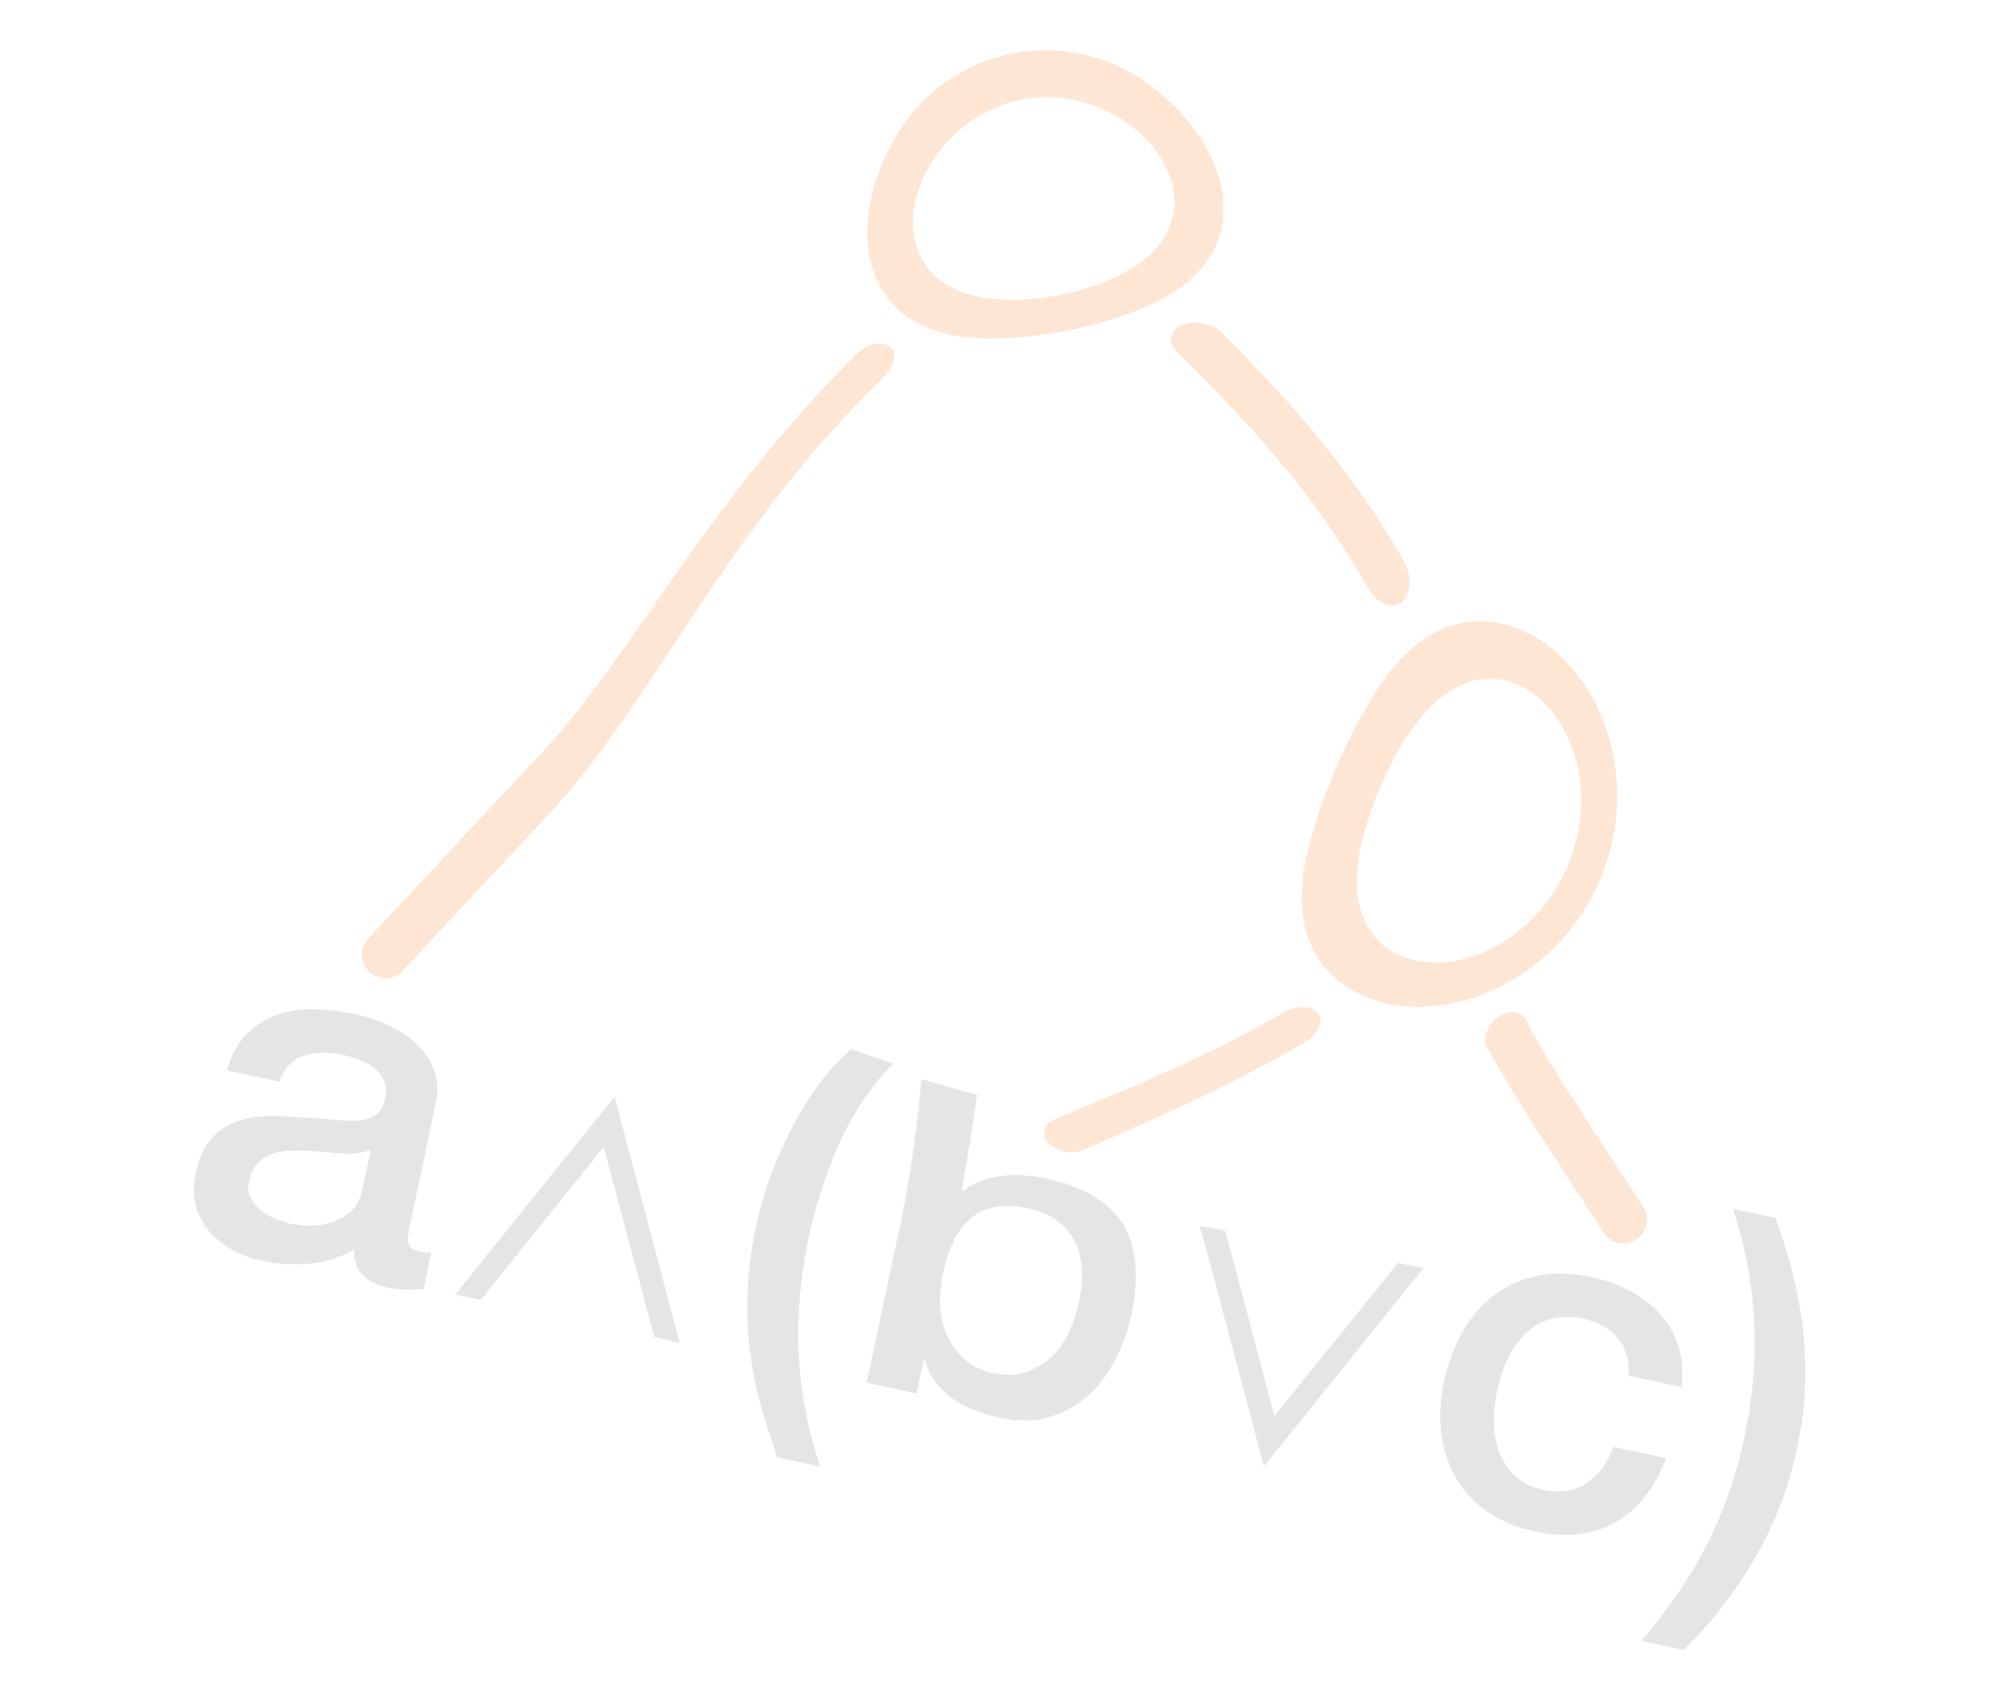
\includegraphics[width=\paperwidth]{fp_images/SyntaxTreeBackground.png}}}
\newcommand{\BgBtInterface}{\usebackgroundtemplate{\transparent{0.1}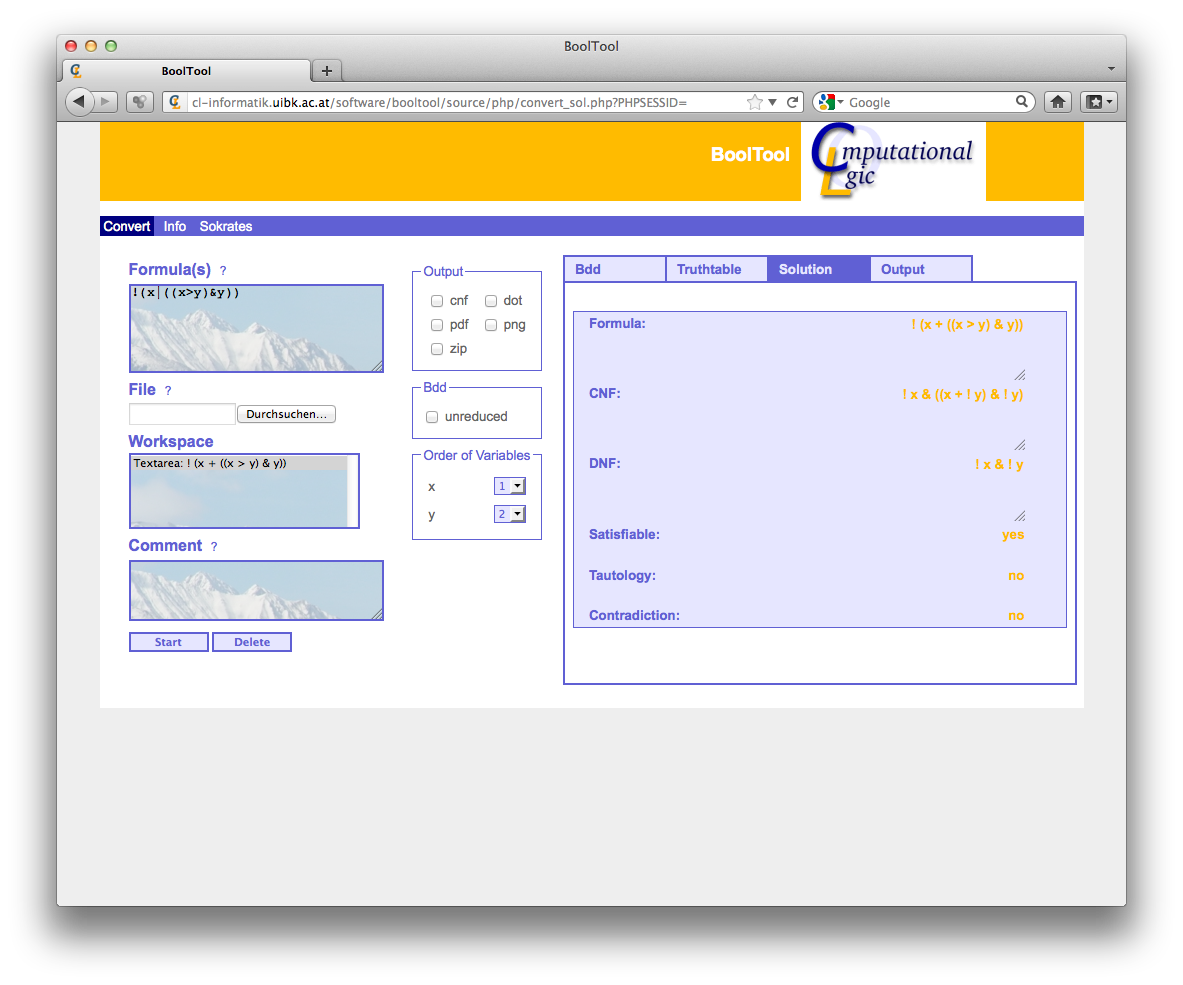
\includegraphics[width=\paperwidth]{fp_images/BoolToolInterface.png}}}

\newcommand{\BgTabB}{\usebackgroundtemplate{\transparent{1}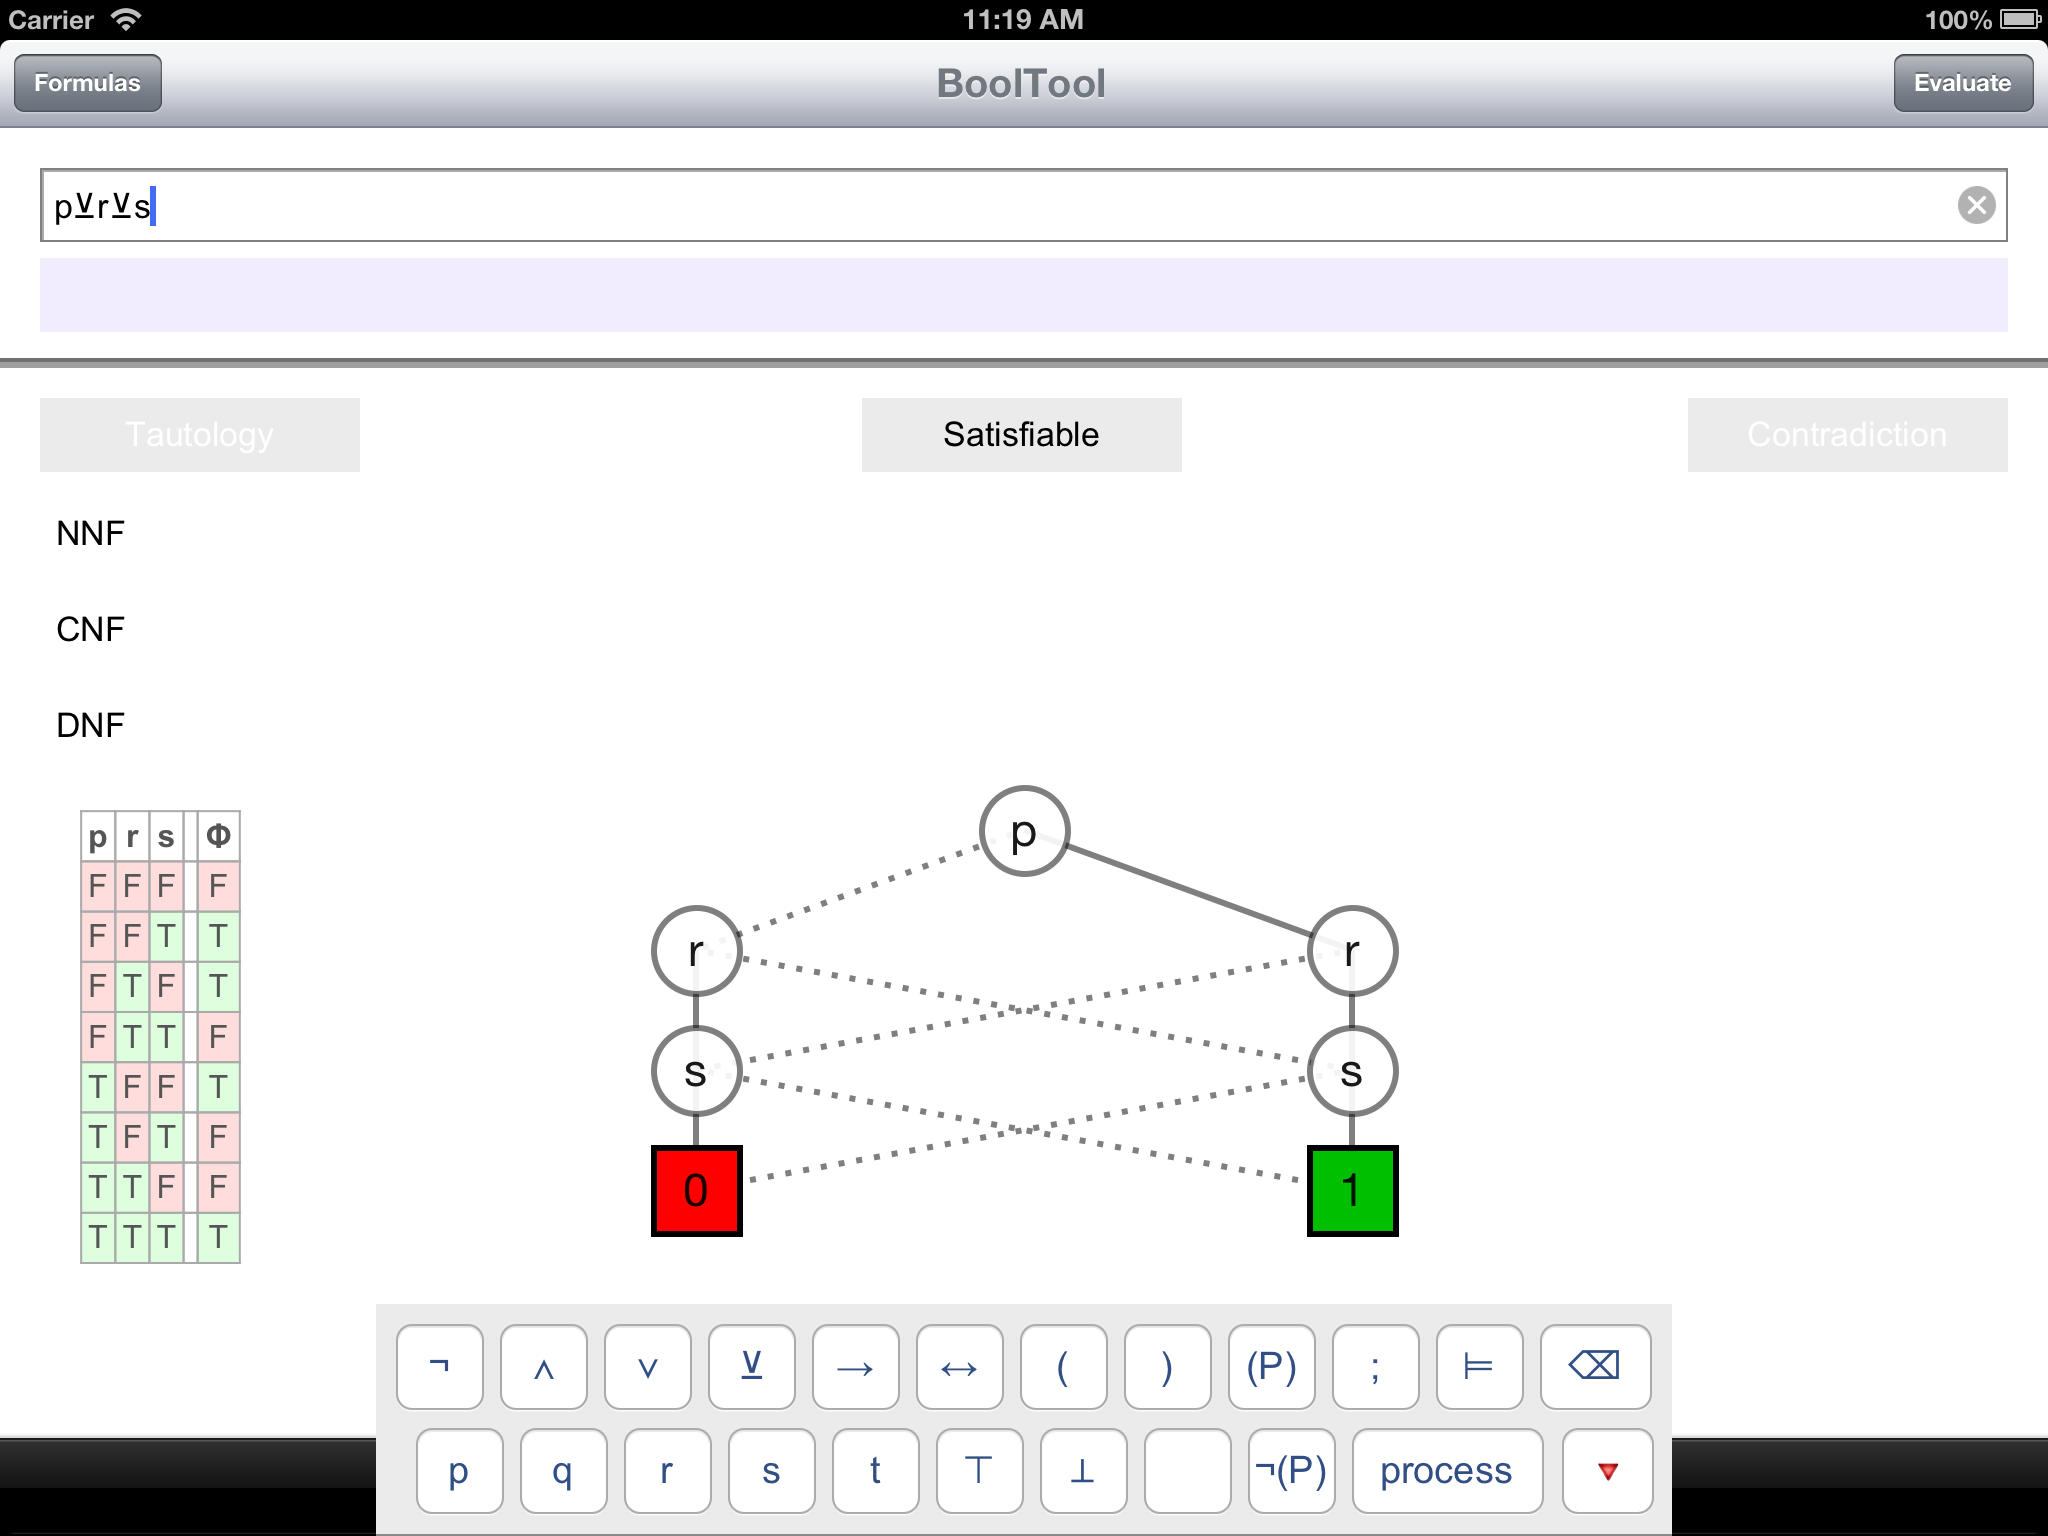
\includegraphics[width=\paperwidth, trim=0 0 0 17mm, clip=true]{fp_images/NyayaTabB1.png}}}
\newcommand{\BgTabE}{\usebackgroundtemplate{\transparent{1}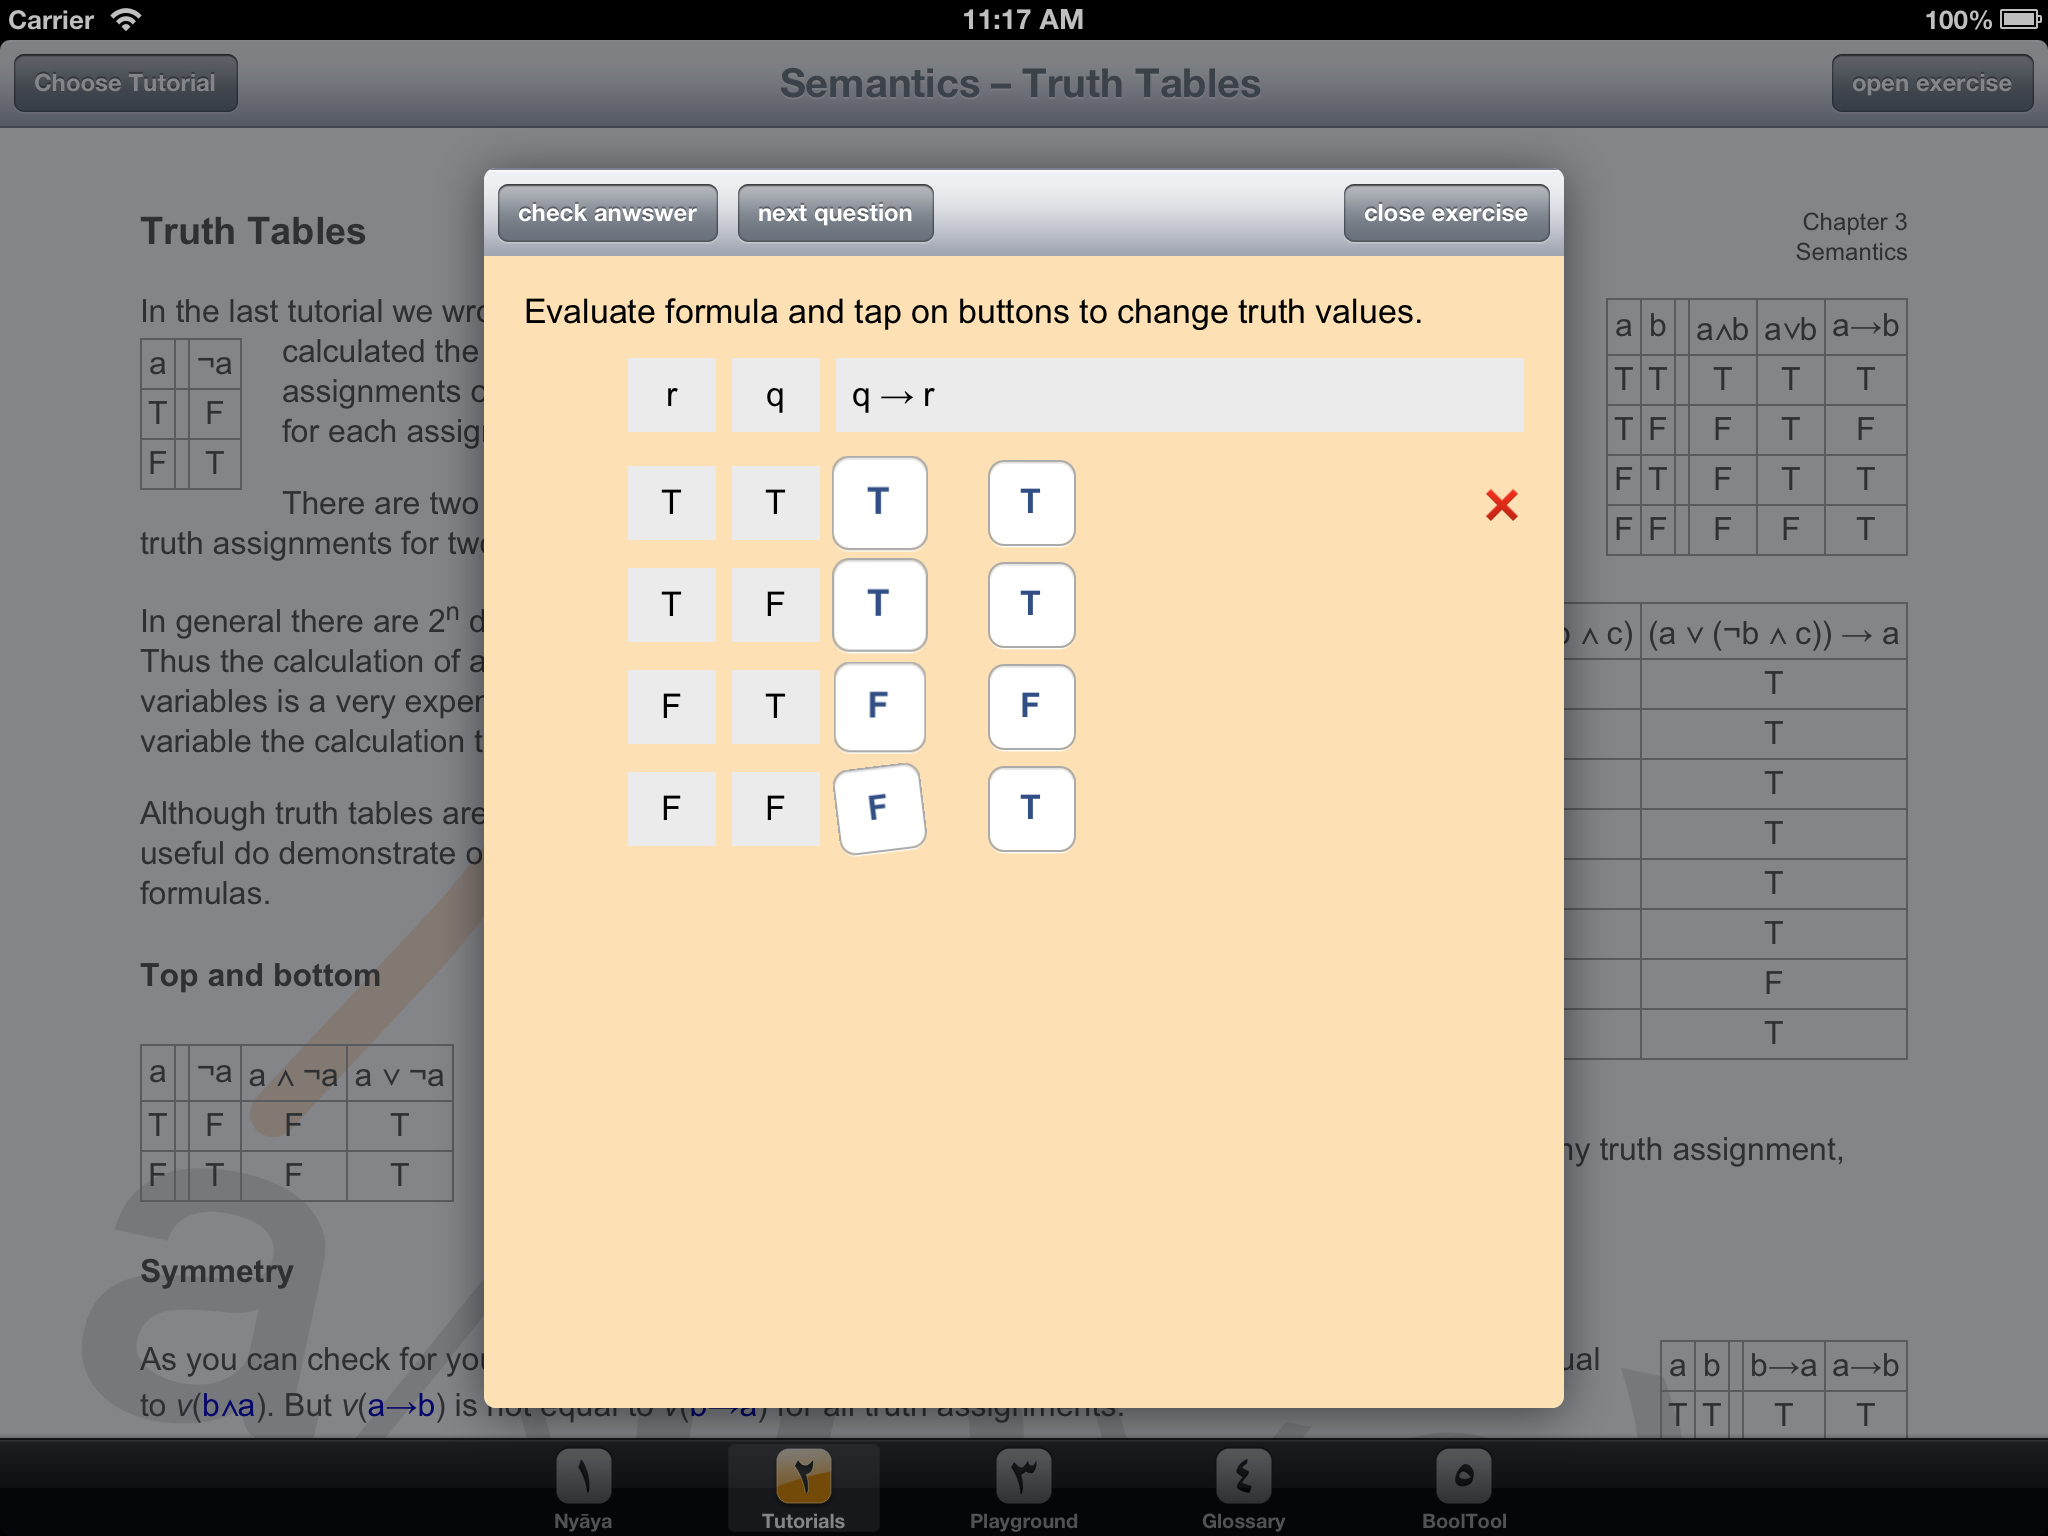
\includegraphics[width=\paperwidth, trim=0 0 0 17mm, clip=true]{fp_images/NyayaTabE1.png}}}
\newcommand{\BgTabG}{\usebackgroundtemplate{\transparent{1}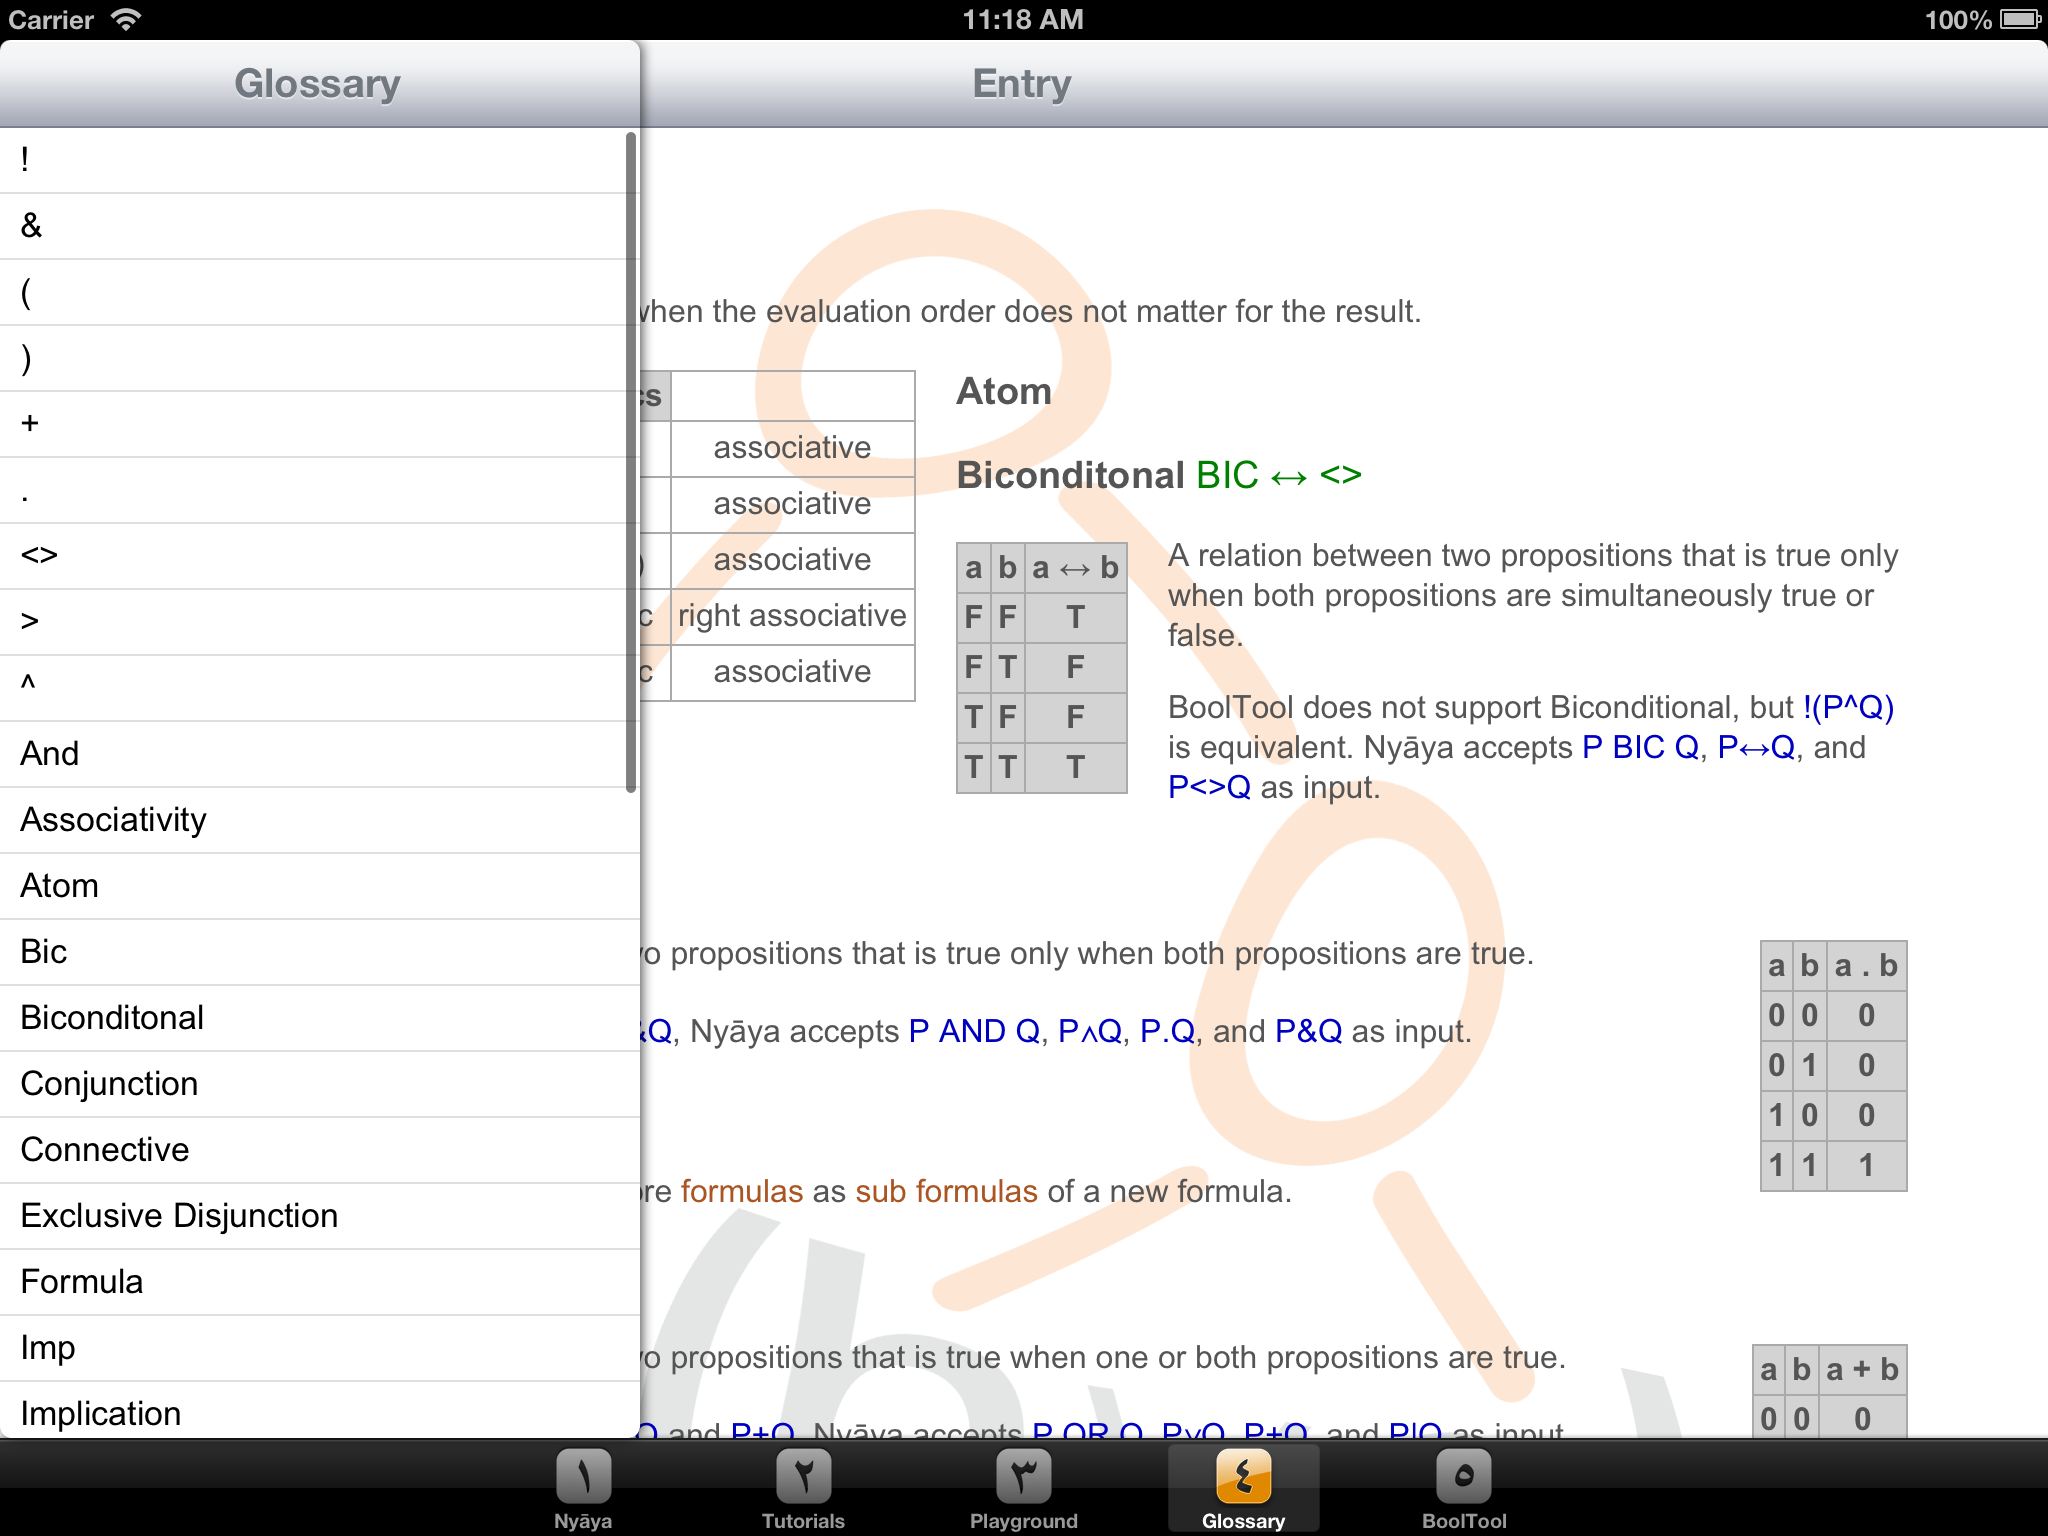
\includegraphics[width=\paperwidth, trim=0 0 0 17mm, clip=true]{fp_images/NyayaTabG1.png}}}
\newcommand{\BgTabN}{\usebackgroundtemplate{\transparent{0.1}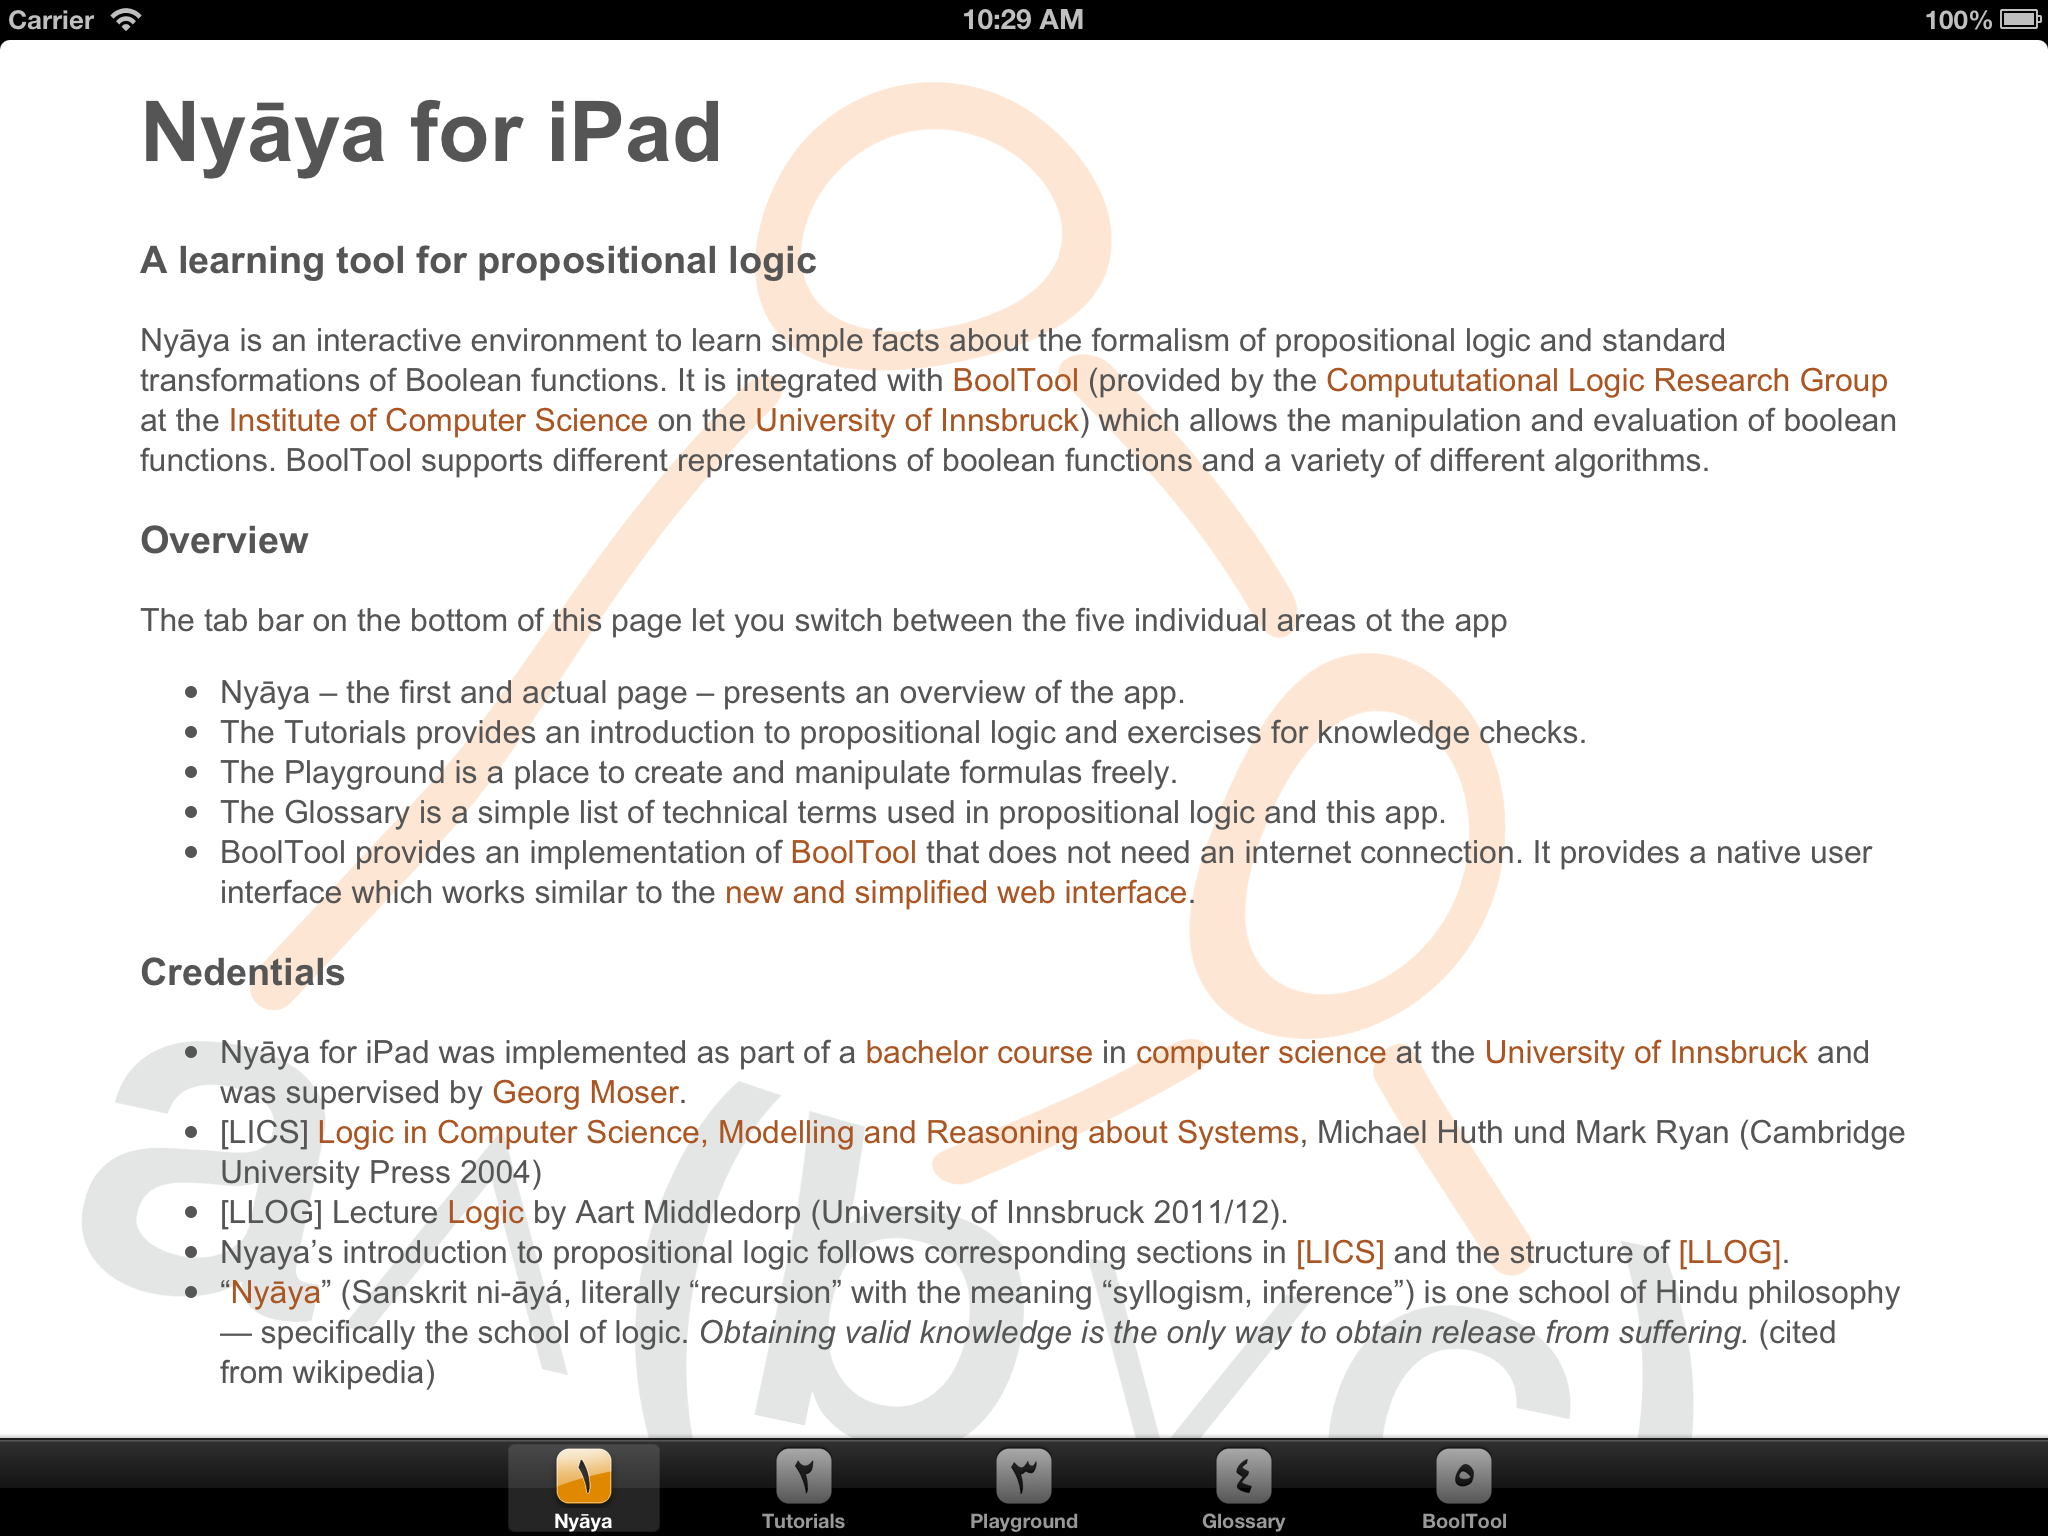
\includegraphics[width=\paperwidth, trim=0 0 0 17mm, clip=true]{fp_images/NyayaTabN1.png}}}
\newcommand{\BgTabP}{\usebackgroundtemplate{\transparent{1}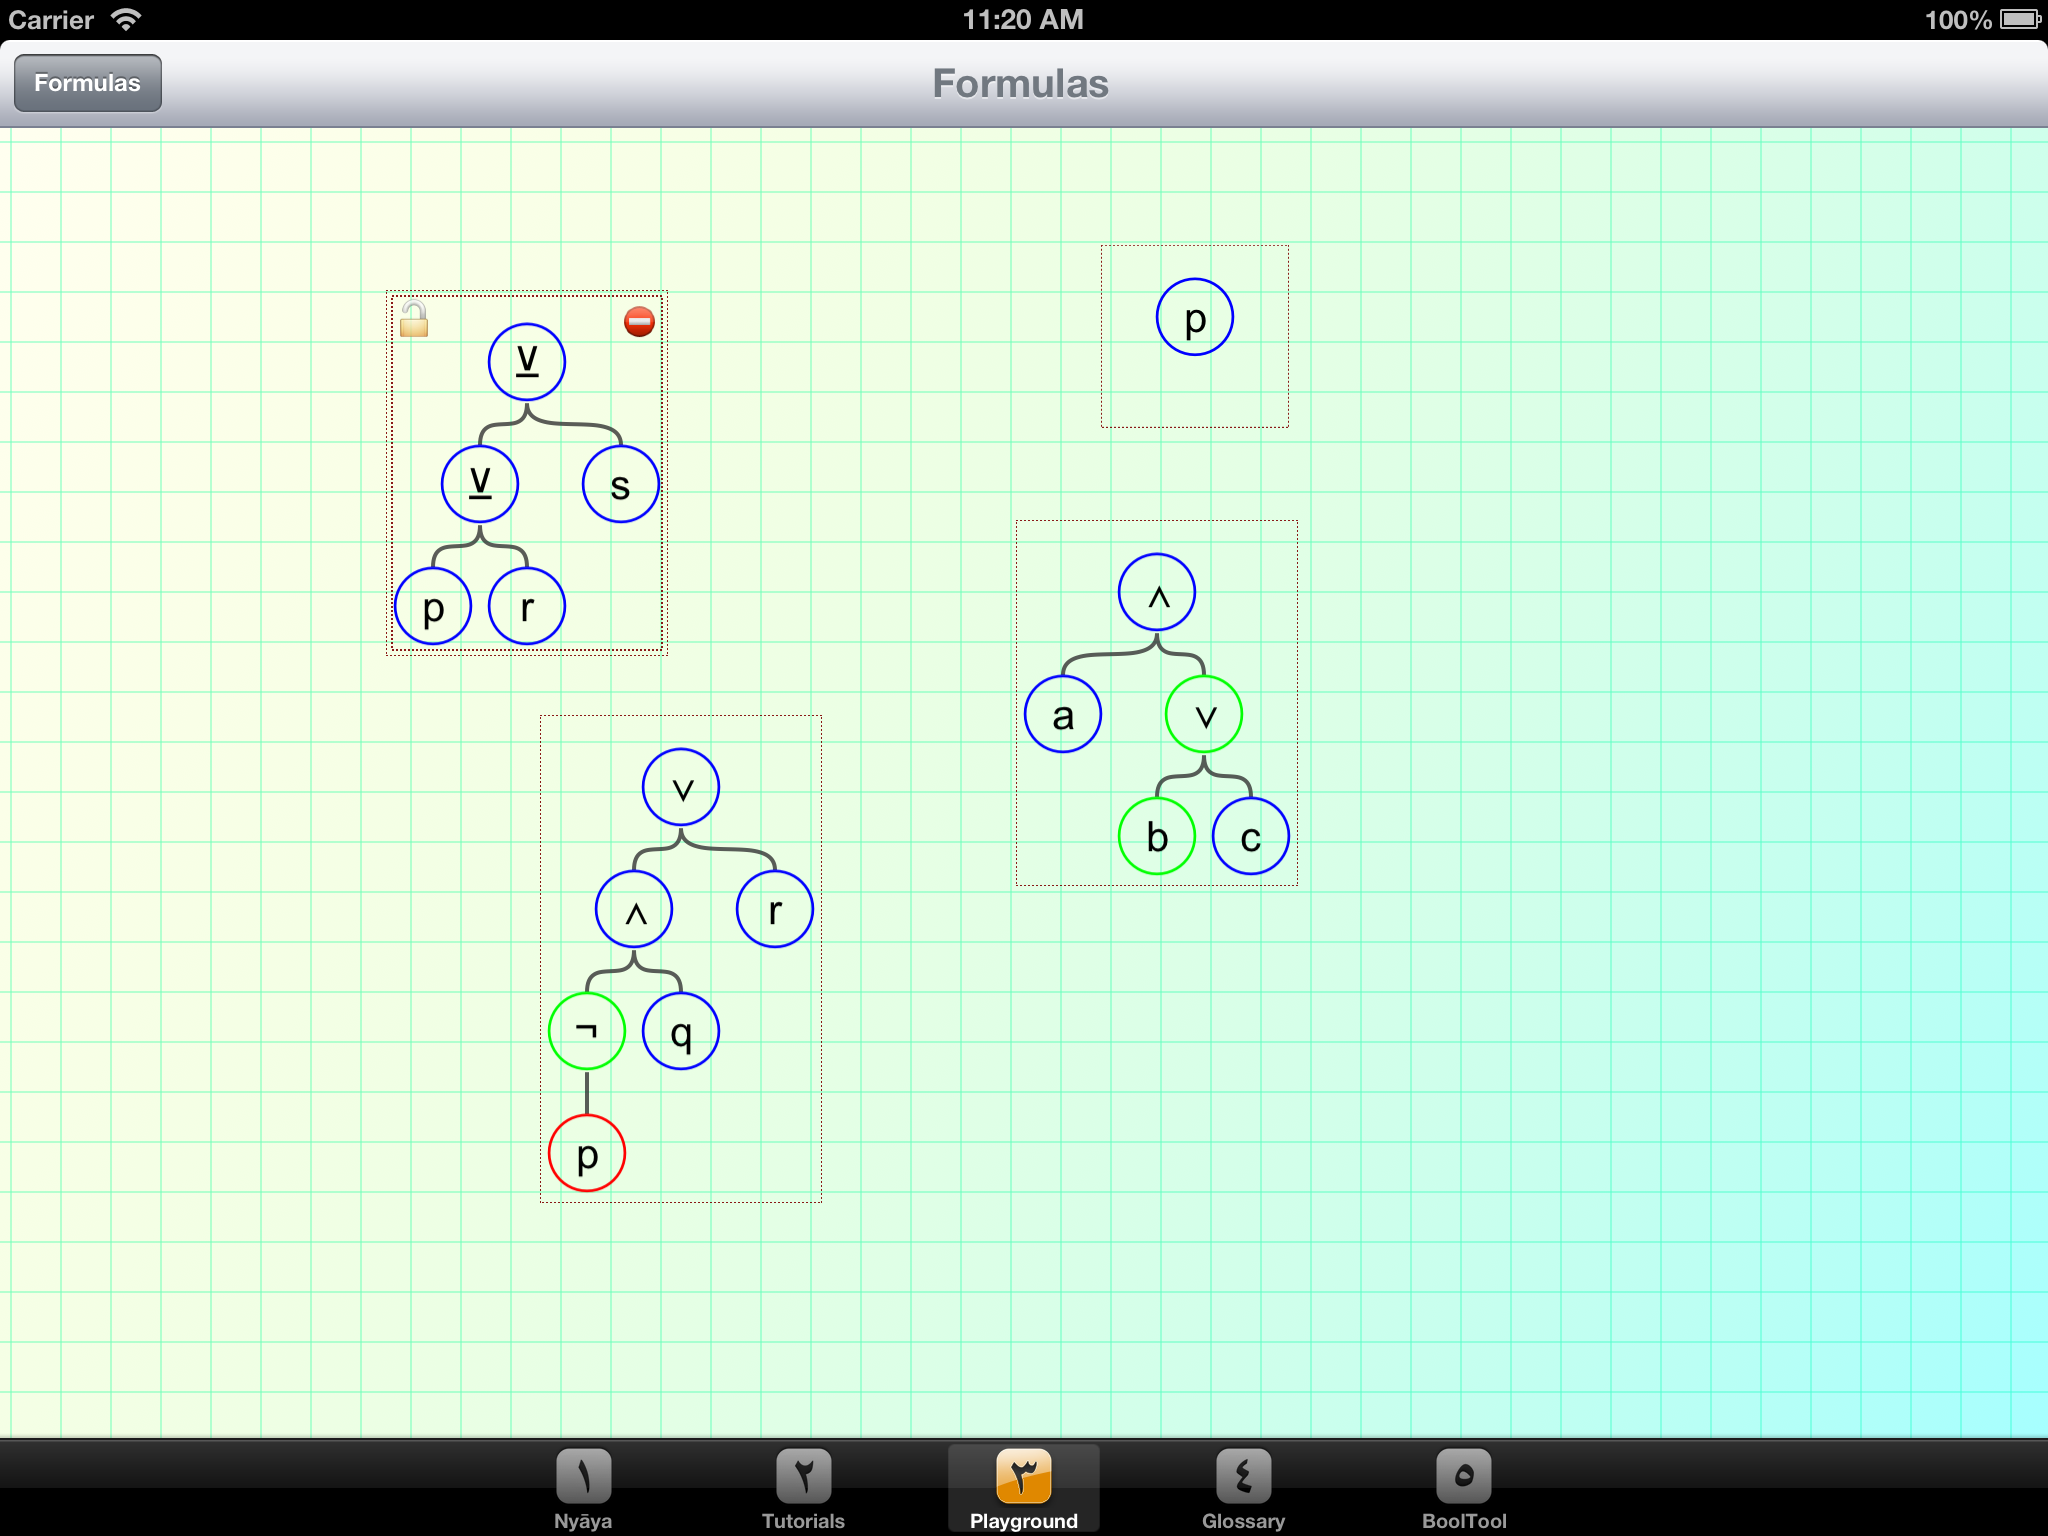
\includegraphics[width=\paperwidth, trim=0 0 0 17mm, clip=true]{fp_images/NyayaTabP1.png}}}
\newcommand{\BgTabT}{\usebackgroundtemplate{\transparent{1}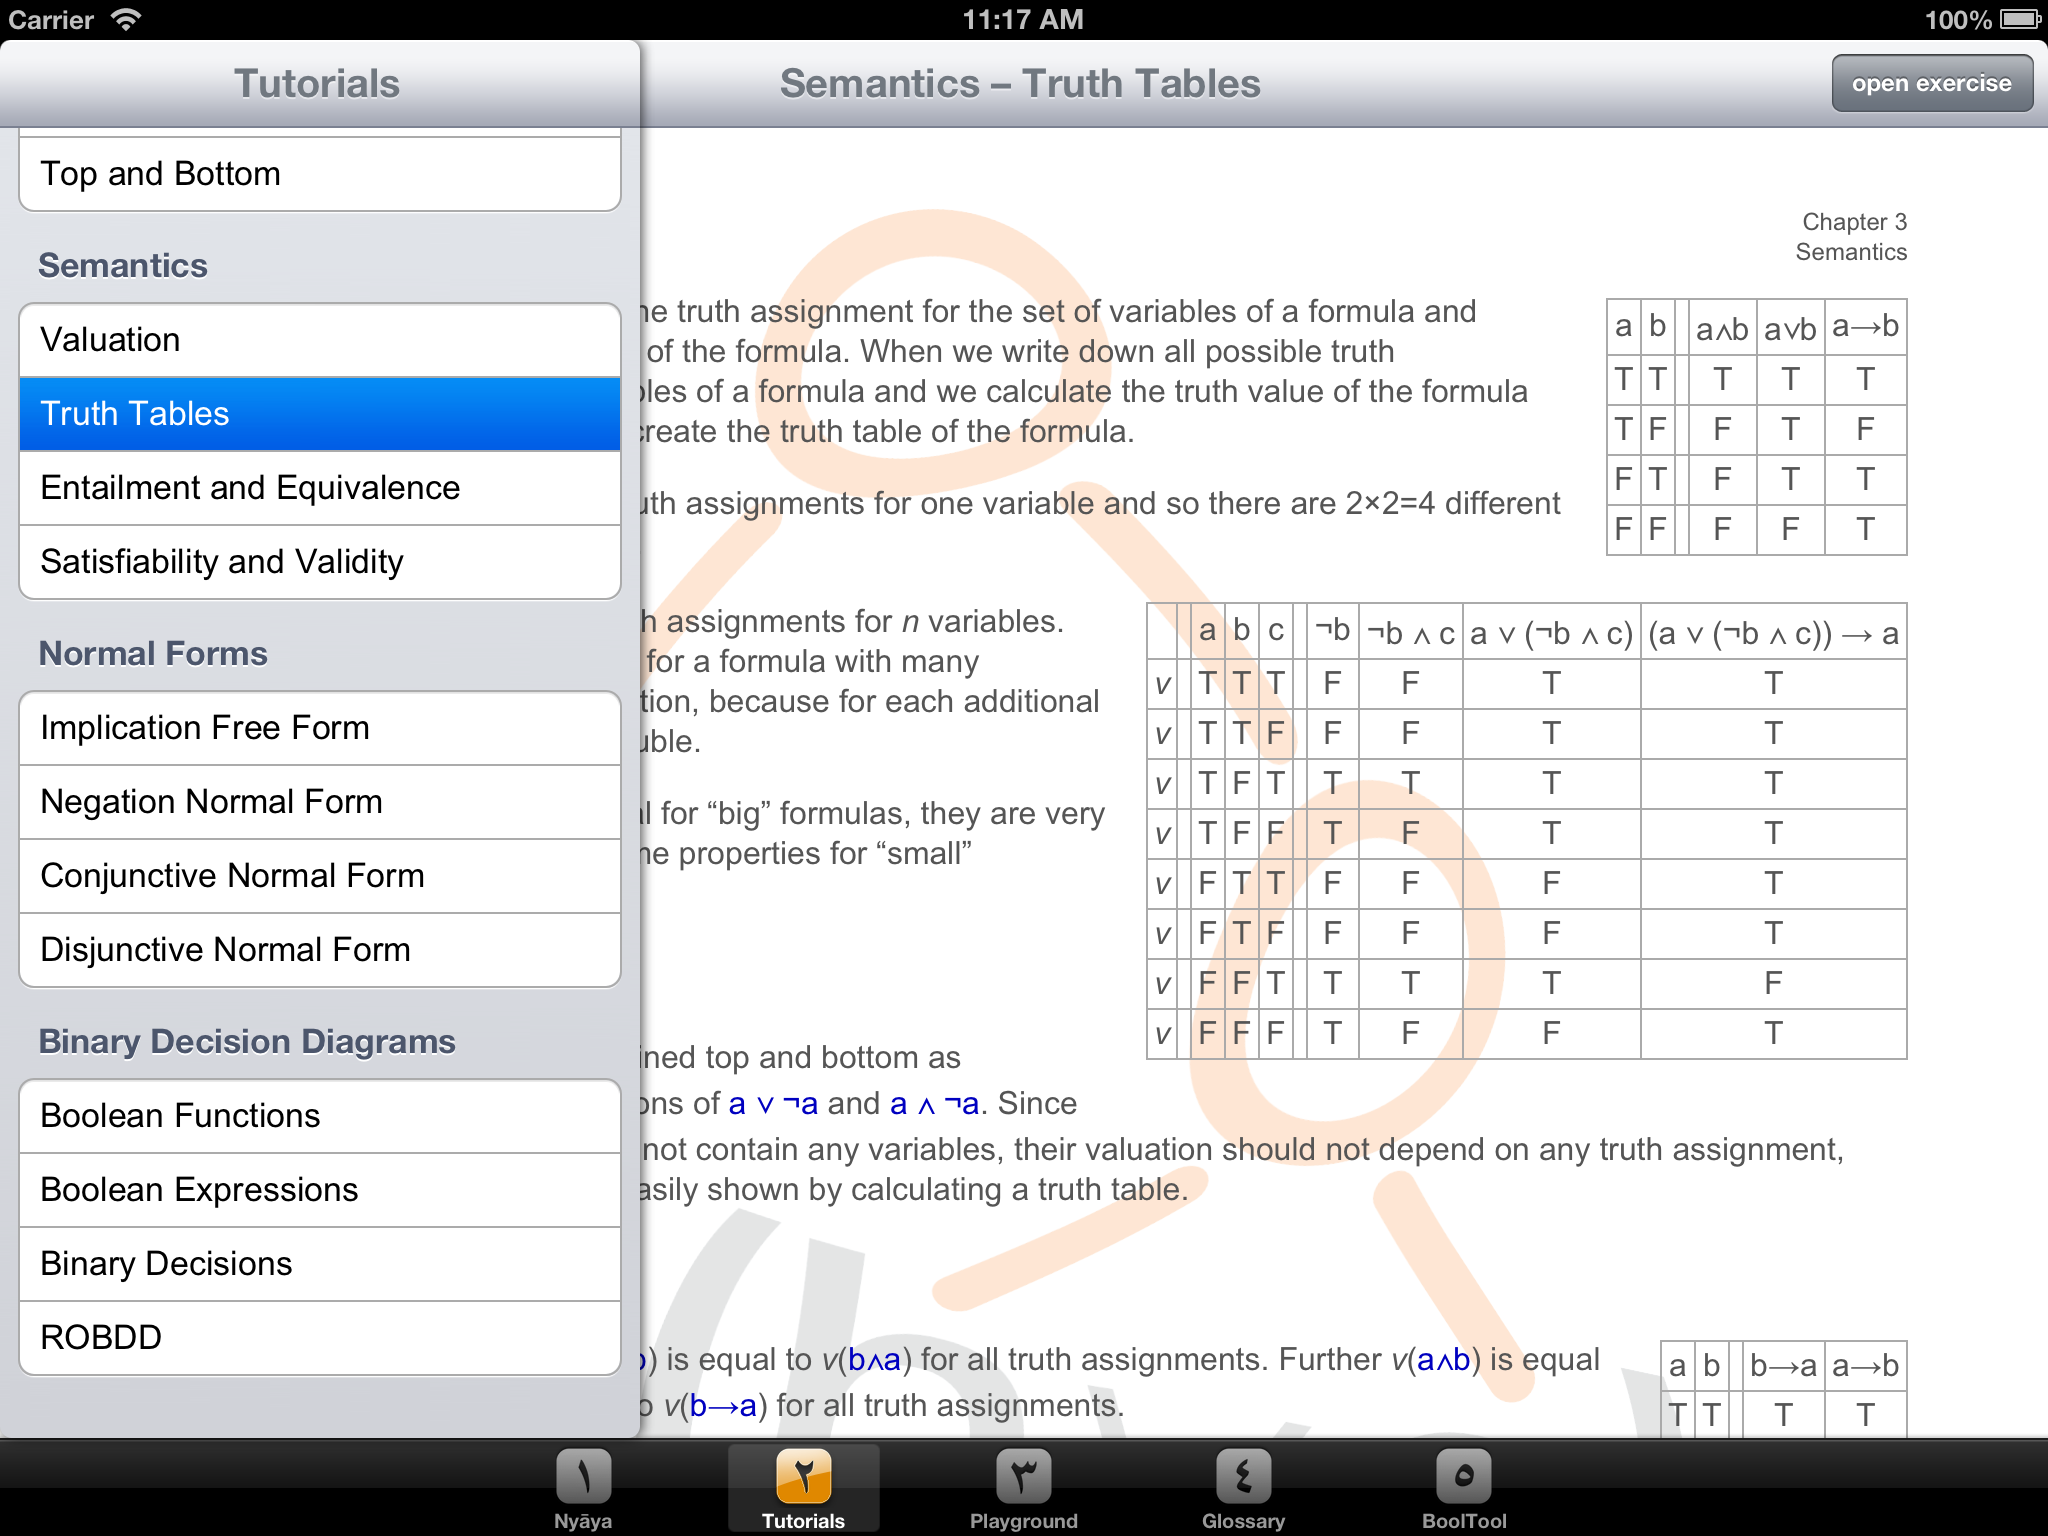
\includegraphics[width=\paperwidth, trim=0 0 0 17mm, clip=true]{fp_images/NyayaTabT1.png}}}





\usebackgroundtemplate{ % 
\includegraphics[width=3cm]{pics/NyayaAppIcon1024.png}}
\vbox to \paperheight{\vspace{2.3cm}\hbox to \paperwidth{\hfil
\includegraphics[width=2.9cm]{pics/NyayaAppIcon1024.png}\hfil}}
}

\title{\Nyaya  for iPad}
\subtitle{Interactive Environment with Bool+Tool \vspace{1.8cm}}
\author{Alexander Maringele}
\institute[UIBK]{}

\date{March 5th, 2013}

\begin{document}

\frame{
\titlepage
Supervisor: Dr. Georg Moser
}




%\section[Outline]{}



% \frame{ \frametitle{Contents} \tableofcontents}

\BgSyntaxTree

% !TEX encoding = UTF-8 Unicode
%

\frame {
	\frametitle{\Nyaya}
	\framesubtitle{Origin and meaning}

\begin{itemize}

	\item<1-> Sanskrit ny-$\bar{\mbox{a}}$yá, literally “recursion”  (Wikipedia)
	\\used in the sense of  “syllogism, inference“. %\footnote{ \tiny \href{http://en.wikipedia.org/wiki/Nyaya}{en.wikipedia.org/wiki/Nyaya}}
	

	\item<2-> One of the schools of Hindu philosophy, 

	specifically the school of logic.%\footnote{ \tiny \href{http://www.iep.utm.edu/nyaya/}{www.iep.utm.edu/nyaya/}}

	\item<3-> \textit{“Obtaining valid knowledge is the only way \newline
	to obtain release from suffering.”} (tenet)
\end{itemize}

% The urge to reason about situations is old.


}
% !TEX encoding = UTF-8 Unicode

\frame {
	\frametitle{Propositional Logic}
	\framesubtitle{Motivation}

The aim of logic in computer science is to develop languages 
to model the situations we encounter as computer science professionals, 
in such way that we can reason about them formally.\footnote{ \tiny
M. Huth and M. Ryan, Logic in Computer Science: Modelling and Reasoning about Systems, 2004}

\vspace{5mm}

\begin{itemize}

\item {\em If wishes were horses beggars would ride.\footnote{ \tiny
Nursery rhyme originating in the 16th century}
}

\item if [wishes are horses] then [beggars ride]

\item $p \rightarrow q$

\item $v(p \rightarrow q) = v(p) \rightarrow v(q) $

\end{itemize}
	
}



%% !TEX encoding = UTF-8 Unicode
%

\frame {
	\frametitle{BoolTool} 
	\framesubtitle{Manipulation and evaluation\\of formulas in propositional logic}


	
\begin{itemize}
\item<1-5,11> BoolTool is powerful
	\begin{itemize}
	\item<2-5> It defines an input syntax for formulas
	\item<3-5> It derives normal forms
	\item<4-5> It computes truth tables and binary decision diagrams
	\item<5-5> It calculates satisfiability, tautologies and contradictions
	\end{itemize}
\item<1,6-> But it is not for beginners.
	\begin{itemize}
	\item<7-10> It does not motivate or explain much.
	\item<8-10> It does not use standard symbols of propositional logic.
	\item<9-10> It does not explain equivalence transformations.
	\item<10-10> It does not define normal forms.
	\end{itemize}
\end{itemize}
	
}

\frame {
	\frametitle{What is \Nyaya?}
	\framesubtitle{Aim}

	Allow the user to learn

\begin{itemize}
	
	\item Formalism of propositional logic
	
	\item Separation of syntax and semantics
	
	\item Normal forms (NNF, CNF, DNF)

	\item Standard transformations of Boolean functions
	
	\item Coherence of different representations
		
	\end{itemize}
in a self-explanatory environment.

}

%\section{Quellen}


\subsection{Concept}
\frame {
	\frametitle{What is \Nyaya?}

	\framesubtitle{Concept}


\Nyaya supports the most effective learning techniques
– steadily learning and practice testing – % \footnote{Dunlosky et al. Improving […{ learning with effective […] techniques: […]} –
with its combination of small bits of learning content  and
seemingly countless exercises. 
	
	\begin{itemize}
	
	\item Tutorials for general concepts and definitions.

	\item Exercises to consolidate the learned concepts and definitions.
	
	\item A Playground to build and transform formulas.
	
	\item A Glossary of technical terms.

	\item Bool+Tool to provide the functionality of BoolTool.


	
\end{itemize}


}

\BgTabN

\subsection{iPad App}
\frame {
	
	\frametitle{What is \Nyaya?}
	\framesubtitle{iPad App}
	%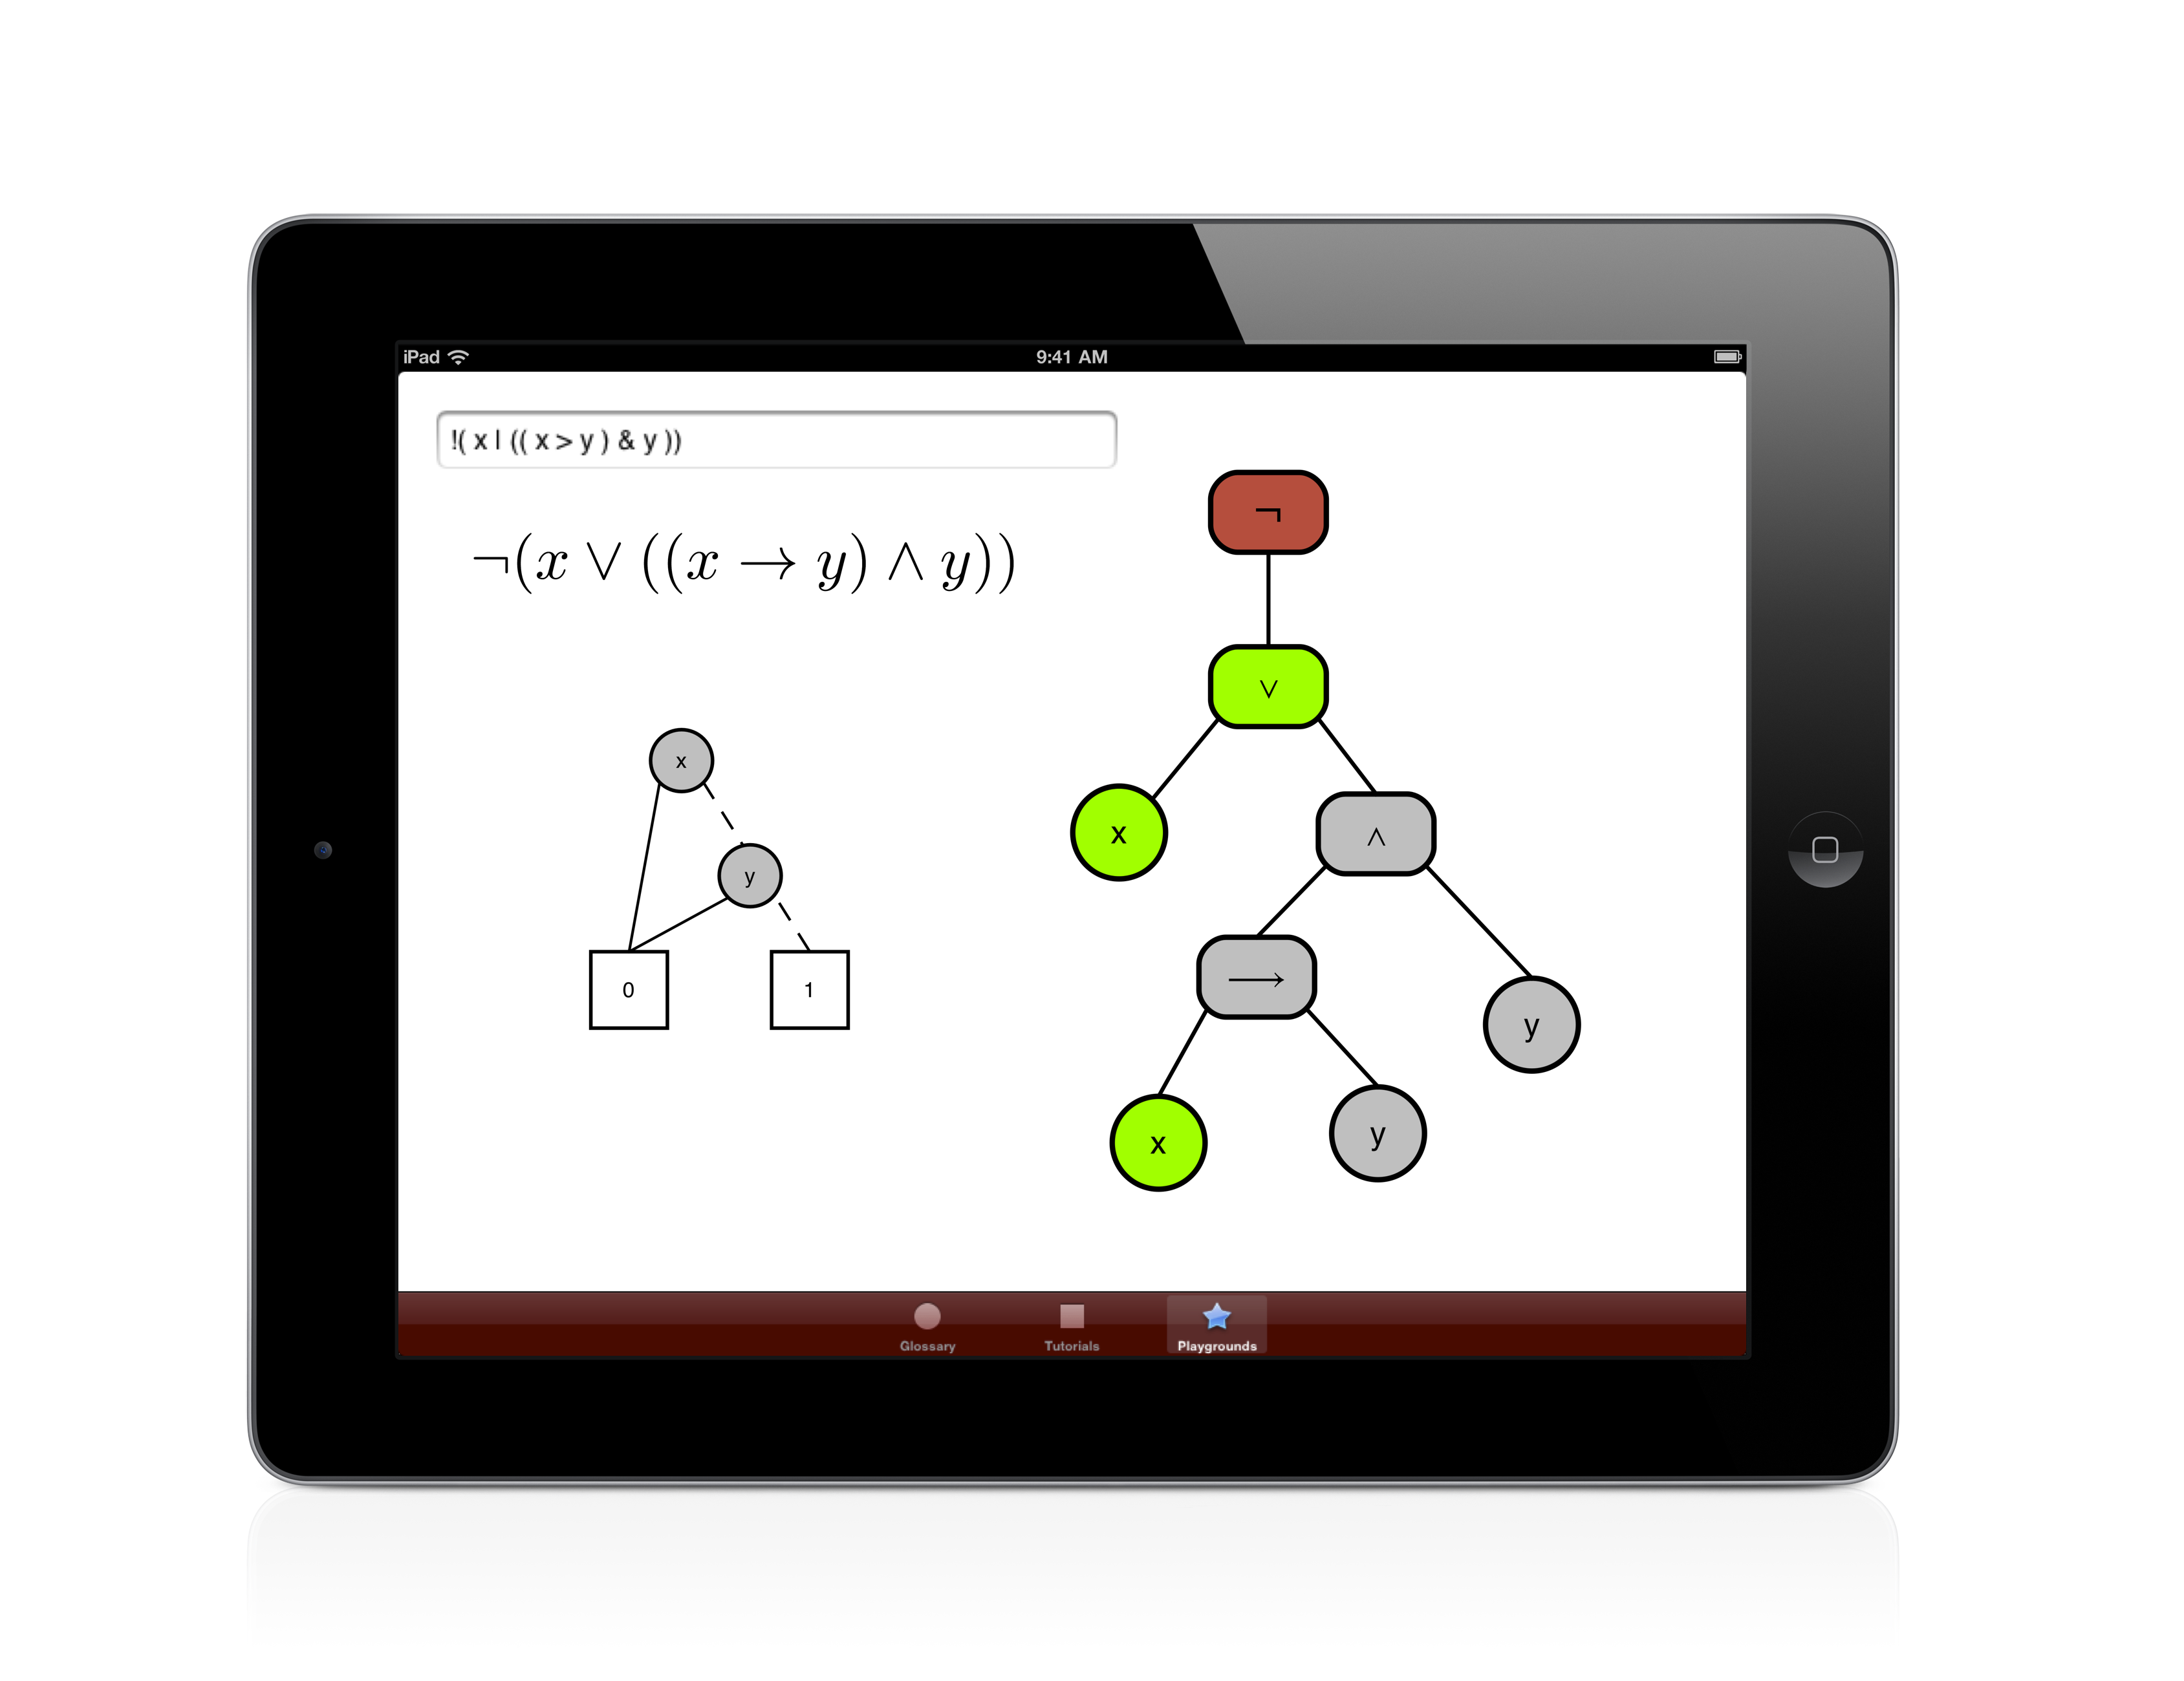
\includegraphics[width=12.2cm,trim=1.5cm 4cm 2cm 2cm]{Images/BoolPad6}

	Popular computing devices
		
	\begin{itemize}
	\item Computers with mice and keyboards
	\item Phones
	\item {\em Tablets with touch interface}
	\end{itemize}
	

	% Tablets with touch interface seams to be the ideal learning environment

	Popular development frameworks for tablets.

	\begin{itemize}
	\item HTML5, CSS3, JavaScript
	% in theory the ideal choice, but in practice theory is more different form practice than in theory.
	\item Android
	\item {\em iOS} 
	\end{itemize}
	
	

}

\BgSyntaxTree

\section{Development Tools and Principles}
\frame{
	\frametitle{Tools and Processes}
	\framesubtitle{}

\begin{itemize}

\item Tools

	\begin{itemize}
	
	\item Xcode, Git, Objective-C, CocoaTouch, Git

	\item Apple Developer Portal, GitHub
	
	\item Interface prototypes, core components
	
	\item Content.

\end{itemize}

\item Principles

\begin{itemize}
	
	\item Fail Fast.

	\item Test-driven development.
	
	\item Refactoring.
	
	\item Use cases.

\end{itemize}
\end{itemize}

}

\section{Implementation}
\frame{
	\frametitle{Implementation}
	\framesubtitle{Model, Views and Controllers}
}

\subsection{Model}
\frame{
	\frametitle{Model}
	%\framesubtitle{Parser}

	\begin{itemize}
	\item BoolTool
		\begin{itemize}
		\item OCaml Sources
		\item Cross-Compiling
		\end{itemize}
	\item Bool+Tool
		\begin{itemize}
		\item Scanner
		\item Parser
		\end{itemize}
	\item Syntax Tree
		\begin{itemize}
		\item Node Cluster
		\item Node Category
		\item Transformations
		\end{itemize}
	\end{itemize}

	
}

%\subsection{Bool+Tool}
\frame {
	\frametitle{Bool+Tool}
	\framesubtitle{Additional features}
%	\begin{itemize}
%	\item Drawbacks
%		\begin{itemize}
%		\item Additional 2 weeks of work
%		\item Slower
%		\item Limits
%		\end{itemize}
%	\item
%		\begin{itemize}
%		\item 
%		\item
%		\end{itemize)
%	\end{itimize}	
%}
}


\subsection{Views}
\frame{
	\frametitle{Views}
	%\framesubtitle{x}	

	\begin{itemize}
	\item SyntaxTreeView
	\item BddView
	\item TruthTableView
	\end{itemize}
}

\subsection{Controllers}
\frame{
	\frametitle{Controllers}
	%\framesubtitle{x}	

	\begin{itemize}
	\item x
	\end{itemize}
}

\BgTabT

\section{Walk-through}
\subsection{Tutorials}
\frame {
	\frametitle{Tutorials}
	\framesubtitle{Walk-through}
}

\BgTabE

\subsection{Exercises}
\frame {
	\frametitle{Exercises}
	\framesubtitle{Walk-through}
}


\BgTabP

\subsection{Playground}
\frame {
	\frametitle{Playground}
	\framesubtitle{Walk-through}
}

\BgTabG

\subsection{Glossary}
\frame {
	\frametitle{Glossary}
	\framesubtitle{Walk-through}
}

\BgTabB

\subsection{BoolTool}
\frame {
	\frametitle{BoolTool}
	\framesubtitle{Walk-through}
}

\BgSyntaxTree

\section{Sources}
\frame{
	\frametitle{Sources}
	
	\begin{itemize}
	\item Huth and Ryan. \textbf{Logic in Computer Science}
	\item Middeldorp. \textbf{Logic}, Lecture 
	\item Gamma, Helm, Johnson, Vlissides. \textbf{Design patterns: elements of reusable object-orientated software}
	\item Louden. \textbf{Compiler Construction: Principles and Practice}
	\item Buck and Yacktman. \textbf{Cocoa Design Patterns}
	\item Apple. \textbf{iOS Developer Documentation}
	% \item OCaml Sourcecode for BoolTool
	% \item Scofield, \textbf{Cross Compiling OCaml to iOS} %, \href{http://psellos.com/ocaml/compile-to-iphone.html}{www.psellos.com}
	
	\end{itemize}
}

%\section{Tools}
%\frame{
%	\frametitle{Tools}
%	
%	\begin{itemize}
%	\item XCode
%	\item Objective C
%	\item Cocoa
%	
%		
%	\end{itemize}
%}


\end{document}
